\section{Posisjonsregulator}\label{sec:posisjonsregulator}
Dersom dere ønsker å tegne kretsskjema med Tikz, finner dere et eksempel i filen
\texttt{kretsskjema.tex} under \texttt{figurer}. Resultatet kan dere se i 
Figur \ref{fig:kretsskjema}. Det er ikke nødvendig å bruke tikz for å tegne kretsskjema, dere kan også bruke andre (mer brukervennlige) programmer. Pass på at 
det er lett å lese kretsskjemaet når dere har satt det inn i rapporten deres!

\begin{figure}[t]
    \centering
    \def\x{4}
\def\y{4}
% Size of the bridge
\def\dx{1.5}
\def\dy{1.5}
\begin{circuitikz}[american voltages]
  \node at (\x+2*\dx,\y) {} ;
  % Voltage source
  \draw (0,0) to [V, l_=$V$,invert]
  (0, \y) to (\x, \y)
  % Left half bridge
  to [R, l_=$R_1$, -] (\x-\dx,\y-\dy) % Top left resistor
  to [R, l_=$R_2$, -] (\x,\y-2*\dy);  % Bottom left resistor
  % Right half bridge
  \draw (\x,\y)
  to [R, l_=$R_3$, -] (\x+\dx, \y-\dy) % Top right resistor
  to [R, l_=$R_T$, -] (\x,\y-2*\dy)  % Bottom left resistor
  % Draw connection to (-) terminal of voltage source
  to (\x, 0) to (0,0);

  % Draw amplifer
  \draw (\x-\dx, \y-\dy) to (\x-1.2*\dx, \y-\dy)
  %\draw (\x-1.5\dx, \y-\dy) 
  to (\x-1.2*\dx, \y-1)
  to[crossing] (\x-1.2*\dx, \y+1) to [short,-*](\x+2*\dx,\y+1);
  \draw (\x+\dx, \y-\dy) to (\x+1.2*\dx, \y-\dy)
  to (\x+1.2*\dx, \y-1)
  to [short,-*](\x+2*\dx,\y-1);
\end{circuitikz}
    \caption{Eksempel på kretsskjema fra Eksamen i TTK4101 2021.}
    \label{fig:kretsskjema}
\end{figure}

Dersom dere eksporterer plots som eps, bruker vi kommandoen \texttt{includegraphics}
for å tegne figuren, som vist i kildekoden. Resultatet er vist i Figur 
\ref{fig:eps_eksempel}.

\begin{figure}[t]
\centering
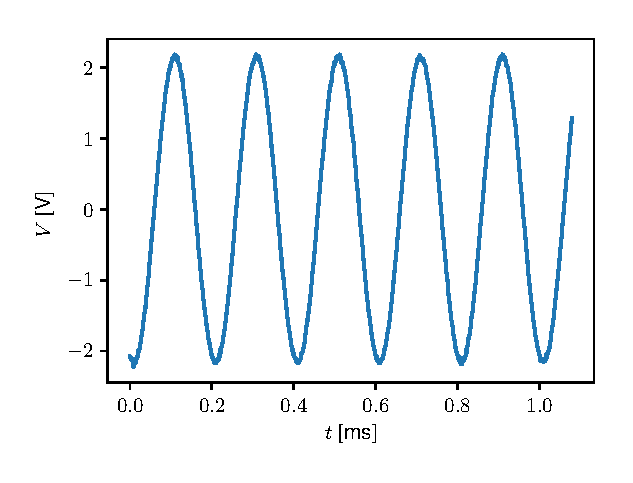
\includegraphics[width=0.4\textwidth]{figurer/eksempel_plott.eps}
\caption{Eksempel på plott med eps-fil. Merk at fontstørrelsen er mindre enn i
resten av dokumentet, ettersom den er styrt av figurstørrelsen når vi laget plottet.}
\label{fig:eps_eksempel}
\end{figure}

Dersom dere eksporterer figurene deres som tikz, bruker vi kommandoen \texttt{\\input}
for å vise figuren. Resultatet er vist i Figur \ref{fig:tikz_eksempel}.
\setlength{\figW}{0.4\textwidth}
\setlength{\figH}{0.35\textwidth}
\begin{figure}[t]
\centering
% This file was created by tikzplotlib v0.9.8.
\begin{tikzpicture}

\definecolor{color0}{rgb}{0.12156862745098,0.466666666666667,0.705882352941177}

\begin{axis}[
height=\figH,
tick align=outside,
tick pos=left,
width=\figW,
x grid style={white!69.0196078431373!black},
xlabel={\(\displaystyle t\) [ms]},
xmin=-0.053988, xmax=1.133748,
xtick style={color=black},
y grid style={white!69.0196078431373!black},
ylabel={\(\displaystyle V\) [V]},
ymin=-2.441895, ymax=2.402835,
ytick style={color=black}
]
\addplot [semithick, color0]
table {%
0 -2.0752
0.000880000000000195 -2.0752
0.00176000000000017 -2.08496
0.00264000000000015 -2.09473
0.00352000000000013 -2.12402
0.00440000000000011 -2.09473
0.00528000000000008 -2.13379
0.00616000000000006 -2.11426
0.00704000000000004 -2.13379
0.00792000000000002 -2.18262
0.0088 -2.22168
0.00968000000000019 -2.13379
0.0105600000000002 -2.17285
0.0114400000000001 -2.14355
0.0123200000000001 -2.11426
0.0132000000000001 -2.10449
0.0140800000000001 -2.10449
0.0149600000000001 -2.16309
0.01584 -2.12402
0.01672 -2.08496
0.0176 -2.0752
0.0184800000000002 -2.06543
0.0193600000000002 -2.06543
0.0202400000000001 -2.06543
0.0211200000000001 -1.97754
0.0220000000000001 -1.97754
0.0228800000000001 -1.99707
0.0237600000000001 -1.94824
0.02464 -1.90918
0.02552 -1.89941
0.0264 -1.86035
0.0272800000000002 -1.81152
0.0281600000000002 -1.80176
0.0290400000000001 -1.7627
0.0299200000000001 -1.72363
0.0308000000000001 -1.7041
0.0316800000000001 -1.65527
0.0325600000000001 -1.61621
0.03344 -1.58691
0.03432 -1.53809
0.0352 -1.46973
0.0360800000000002 -1.45996
0.0369600000000002 -1.40137
0.0378400000000001 -1.40137
0.0387200000000001 -1.29395
0.0396000000000001 -1.27441
0.0404800000000001 -1.21582
0.04136 -1.19629
0.04224 -1.1084
0.04312 -1.06934
0.0440000000000002 -1.01074
0.0448800000000002 -0.991211
0.0457600000000002 -0.913086
0.0466400000000001 -0.825195
0.0475200000000001 -0.795898
0.0484000000000001 -0.717773
0.0492800000000001 -0.678711
0.0501600000000001 -0.610352
0.05104 -0.561523
0.05192 -0.50293
0.0528000000000002 -0.43457
0.0536800000000002 -0.424805
0.0545600000000002 -0.327148
0.0554400000000001 -0.249023
0.0563200000000001 -0.219727
0.0572000000000001 -0.151367
0.0580800000000001 -0.112305
0.05896 -0.0537109
0.05984 0.0244141
0.06072 0.0634766
0.0616000000000002 0.170898
0.0624800000000002 0.180664
0.0633600000000002 0.268555
0.0642400000000001 0.288086
0.0651200000000001 0.366211
0.0660000000000001 0.415039
0.0668800000000001 0.493164
0.06776 0.512695
0.06864 0.571289
0.06952 0.668945
0.0704000000000002 0.727539
0.0712800000000002 0.756836
0.0721600000000002 0.795898
0.0730400000000001 0.883789
0.0739200000000001 0.961914
0.0748000000000001 0.981445
0.0756800000000001 1.02051
0.07656 1.09863
0.07744 1.1377
0.07832 1.18652
0.0792000000000002 1.24512
0.0800800000000002 1.30371
0.0809600000000001 1.32324
0.0818400000000001 1.37207
0.0827200000000001 1.4209
0.0836000000000001 1.48926
0.0844800000000001 1.52832
0.08536 1.54785
0.08624 1.58691
0.08712 1.65527
0.0880000000000002 1.6748
0.0888800000000002 1.69434
0.0897600000000001 1.77246
0.0906400000000001 1.7627
0.0915200000000001 1.80176
0.0924000000000001 1.86035
0.0932800000000001 1.86035
0.09416 1.91895
0.09504 1.90918
0.09592 1.96777
0.0968000000000002 1.95801
0.0976800000000002 2.02637
0.0985600000000001 1.9873
0.0994400000000001 2.02637
0.10032 2.0459
0.1012 2.0752
0.10208 2.09473
0.10296 2.11426
0.10384 2.12402
0.10472 2.14355
0.1056 2.11426
0.10648 2.12402
0.10736 2.14355
0.10824 2.17285
0.10912 2.18262
0.11 2.14355
0.11088 2.17285
0.11176 2.17285
0.11264 2.14355
0.11352 2.12402
0.1144 2.10449
0.11528 2.11426
0.11616 2.14355
0.11704 2.09473
0.11792 2.0752
0.1188 2.06543
0.11968 2.02637
0.12056 2.02637
0.12144 2.00684
0.12232 2.03613
0.1232 1.94824
0.12408 1.93848
0.12496 1.91895
0.12584 1.87012
0.12672 1.89941
0.1276 1.82129
0.12848 1.84082
0.12936 1.78223
0.13024 1.7334
0.13112 1.68457
0.132 1.60645
0.13288 1.60645
0.13376 1.53809
0.13464 1.53809
0.13552 1.48926
0.1364 1.45996
0.13728 1.40137
0.13816 1.3623
0.13904 1.28418
0.13992 1.27441
0.1408 1.18652
0.14168 1.16699
0.14256 1.1084
0.14344 1.0498
0.14432 0.991211
0.1452 0.942383
0.14608 0.922852
0.14696 0.854492
0.14784 0.786133
0.14872 0.756836
0.1496 0.649414
0.15048 0.600586
0.15136 0.561523
0.15224 0.512695
0.15312 0.454102
0.154 0.366211
0.15488 0.297852
0.15576 0.27832
0.15664 0.219727
0.15752 0.131836
0.1584 0.0439453
0.15928 0.0439453
0.16016 -0.0341797
0.16104 -0.102539
0.16192 -0.141602
0.1628 -0.229492
0.16368 -0.27832
0.16456 -0.317383
0.16544 -0.375977
0.16632 -0.463867
0.1672 -0.561523
0.16808 -0.571289
0.16896 -0.610352
0.16984 -0.688477
0.17072 -0.737305
0.1716 -0.825195
0.17248 -0.854492
0.17336 -0.913086
0.17424 -0.961914
0.17512 -1.03027
0.176 -1.02051
0.17688 -1.12793
0.17776 -1.16699
0.17864 -1.23535
0.17952 -1.26465
0.1804 -1.31348
0.18128 -1.3623
0.18216 -1.4209
0.18304 -1.44043
0.18392 -1.48926
0.1848 -1.51855
0.18568 -1.59668
0.18656 -1.58691
0.18744 -1.65527
0.18832 -1.64551
0.1892 -1.72363
0.19008 -1.75293
0.19096 -1.79199
0.19184 -1.82129
0.19272 -1.86035
0.1936 -1.89941
0.19448 -1.88965
0.19536 -1.93848
0.19624 -1.95801
0.19712 -1.96777
0.198 -2.00684
0.19888 -2.0459
0.19976 -2.0459
0.20064 -2.08496
0.20152 -2.0752
0.2024 -2.11426
0.20328 -2.11426
0.20416 -2.11426
0.20504 -2.11426
0.20592 -2.12402
0.2068 -2.17285
0.20768 -2.15332
0.20856 -2.15332
0.20944 -2.13379
0.21032 -2.17285
0.2112 -2.14355
0.21208 -2.15332
0.21296 -2.14355
0.21384 -2.14355
0.21472 -2.11426
0.2156 -2.11426
0.21648 -2.12402
0.21736 -2.11426
0.21824 -2.0459
0.21912 -2.08496
0.22 -2.02637
0.22088 -1.97754
0.22176 -2.0166
0.22264 -1.9873
0.22352 -1.93848
0.2244 -1.92871
0.22528 -1.90918
0.22616 -1.88965
0.22704 -1.81152
0.22792 -1.81152
0.2288 -1.78223
0.22968 -1.74316
0.23056 -1.71387
0.23144 -1.66504
0.23232 -1.61621
0.2332 -1.59668
0.23408 -1.55762
0.23496 -1.52832
0.23584 -1.46973
0.23672 -1.45996
0.2376 -1.38184
0.23848 -1.34277
0.23936 -1.29395
0.24024 -1.23535
0.24112 -1.20605
0.242 -1.1377
0.24288 -1.0791
0.24376 -1.04004
0.24464 -0.97168
0.24552 -0.942383
0.2464 -0.874023
0.24728 -0.844727
0.24816 -0.766602
0.24904 -0.688477
0.24992 -0.678711
0.2508 -0.600586
0.25168 -0.551758
0.25256 -0.483398
0.25344 -0.43457
0.25432 -0.375977
0.2552 -0.297852
0.25608 -0.239258
0.25696 -0.180664
0.25784 -0.102539
0.25872 -0.0634766
0.2596 0.00488281
0.26048 0.0537109
0.26136 0.0732422
0.26224 0.141602
0.26312 0.249023
0.264 0.288086
0.26488 0.336914
0.26576 0.395508
0.26664 0.473633
0.26752 0.541992
0.2684 0.600586
0.26928 0.639648
0.27016 0.688477
0.27104 0.74707
0.27192 0.805664
0.2728 0.864258
0.27368 0.952148
0.27456 0.97168
0.27544 1.01074
0.27632 1.06934
0.2772 1.1377
0.27808 1.18652
0.27896 1.23535
0.27984 1.26465
0.28072 1.32324
0.2816 1.38184
0.28248 1.4502
0.28336 1.45996
0.28424 1.50879
0.28512 1.51855
0.286 1.60645
0.28688 1.60645
0.28776 1.68457
0.28864 1.69434
0.28952 1.7627
0.2904 1.75293
0.29128 1.82129
0.29216 1.87012
0.29304 1.88965
0.29392 1.89941
0.2948 1.95801
0.29568 1.96777
0.29656 1.9873
0.29744 1.97754
0.29832 2.0459
0.2992 2.03613
0.30008 2.06543
0.30096 2.0459
0.30184 2.06543
0.30272 2.11426
0.3036 2.11426
0.30448 2.13379
0.30536 2.14355
0.30624 2.16309
0.30712 2.11426
0.308 2.14355
0.30888 2.18262
0.30976 2.17285
0.31064 2.16309
0.31152 2.16309
0.3124 2.16309
0.31328 2.11426
0.31416 2.16309
0.31504 2.10449
0.31592 2.09473
0.3168 2.11426
0.31768 2.09473
0.31856 2.06543
0.31944 2.0459
0.32032 2.0166
0.3212 2.00684
0.32208 1.9873
0.32296 1.97754
0.32384 1.95801
0.32472 1.91895
0.3256 1.87012
0.32648 1.87988
0.32736 1.84082
0.32824 1.82129
0.32912 1.7627
0.33 1.72363
0.33088 1.69434
0.33176 1.68457
0.33264 1.63574
0.33352 1.58691
0.3344 1.53809
0.33528 1.48926
0.33616 1.44043
0.33704 1.4502
0.33792 1.35254
0.3388 1.35254
0.33968 1.27441
0.34056 1.21582
0.34144 1.18652
0.34232 1.1084
0.3432 1.0791
0.34408 1.01074
0.34496 1.00098
0.34584 0.874023
0.34672 0.854492
0.3476 0.825195
0.34848 0.727539
0.34936 0.698242
0.35024 0.639648
0.35112 0.600586
0.352 0.522461
0.35288 0.473633
0.35376 0.415039
0.35464 0.356445
0.35552 0.288086
0.3564 0.239258
0.35728 0.170898
0.35816 0.102539
0.35904 0.0537109
0.35992 0.0146484
0.3608 -0.0537109
0.36168 -0.141602
0.36256 -0.200195
0.36344 -0.288086
0.36432 -0.27832
0.3652 -0.34668
0.36608 -0.415039
0.36696 -0.50293
0.36784 -0.541992
0.36872 -0.639648
0.3696 -0.620117
0.37048 -0.737305
0.37136 -0.727539
0.37224 -0.844727
0.37312 -0.913086
0.374 -0.913086
0.37488 -0.952148
0.37576 -1.0498
0.37664 -1.0791
0.37752 -1.12793
0.3784 -1.15723
0.37928 -1.24512
0.38016 -1.26465
0.38104 -1.33301
0.38192 -1.3916
0.3828 -1.4502
0.38368 -1.45996
0.38456 -1.50879
0.38544 -1.56738
0.38632 -1.57715
0.3872 -1.64551
0.38808 -1.66504
0.38896 -1.7041
0.38984 -1.7334
0.39072 -1.77246
0.3916 -1.83105
0.39248 -1.84082
0.39336 -1.87988
0.39424 -1.90918
0.39512 -1.94824
0.396 -1.9873
0.39688 -1.96777
0.39776 -1.99707
0.39864 -2.0166
0.39952 -2.05566
0.4004 -2.02637
0.40128 -2.0752
0.40216 -2.08496
0.40304 -2.09473
0.40392 -2.10449
0.4048 -2.10449
0.40568 -2.14355
0.40656 -2.14355
0.40744 -2.11426
0.40832 -2.16309
0.4092 -2.17285
0.41008 -2.15332
0.41096 -2.17285
0.41184 -2.17285
0.41272 -2.14355
0.4136 -2.14355
0.41448 -2.13379
0.41536 -2.12402
0.41624 -2.11426
0.41712 -2.09473
0.418 -2.08496
0.41888 -2.02637
0.41976 -2.02637
0.42064 -2.02637
0.42152 -2.0166
0.4224 -1.97754
0.42328 -1.96777
0.42416 -1.94824
0.42504 -1.88965
0.42592 -1.89941
0.4268 -1.86035
0.42768 -1.82129
0.42856 -1.79199
0.42944 -1.7627
0.43032 -1.71387
0.4312 -1.64551
0.43208 -1.58691
0.43296 -1.54785
0.43384 -1.56738
0.43472 -1.52832
0.4356 -1.50879
0.43648 -1.4209
0.43736 -1.40137
0.43824 -1.35254
0.43912 -1.28418
0.44 -1.23535
0.44088 -1.22559
0.44176 -1.11816
0.44264 -1.0791
0.44352 -1.05957
0.4444 -0.981445
0.44528 -0.922852
0.44616 -0.874023
0.44704 -0.834961
0.44792 -0.795898
0.4488 -0.708008
0.44968 -0.649414
0.45056 -0.629883
0.45144 -0.541992
0.45232 -0.512695
0.4532 -0.43457
0.45408 -0.366211
0.45496 -0.317383
0.45584 -0.258789
0.45672 -0.219727
0.4576 -0.131836
0.45848 -0.0927734
0.45936 -0.0146484
0.46024 0.0439453
0.46112 0.112305
0.462 0.12207
0.46288 0.209961
0.46376 0.239258
0.46464 0.336914
0.46552 0.366211
0.4664 0.463867
0.46728 0.532227
0.46816 0.571289
0.46904 0.610352
0.46992 0.708008
0.4708 0.698242
0.47168 0.805664
0.47256 0.81543
0.47344 0.90332
0.47432 0.961914
0.4752 1.00098
0.47608 1.0498
0.47696 1.08887
0.47784 1.14746
0.47872 1.22559
0.4796 1.25488
0.48048 1.34277
0.48136 1.35254
0.48224 1.38184
0.48312 1.4209
0.484 1.48926
0.48488 1.52832
0.48576 1.58691
0.48664 1.58691
0.48752 1.6748
0.4884 1.6748
0.48928 1.74316
0.49016 1.7334
0.49104 1.79199
0.49192 1.78223
0.4928 1.84082
0.49368 1.88965
0.49456 1.92871
0.49544 1.93848
0.49632 1.96777
0.4972 2.00684
0.49808 2.0459
0.49896 2.06543
0.49984 2.0752
0.50072 2.0459
0.5016 2.08496
0.50248 2.08496
0.50336 2.14355
0.50424 2.13379
0.50512 2.15332
0.506 2.11426
0.50688 2.15332
0.50776 2.14355
0.50864 2.15332
0.50952 2.15332
0.5104 2.13379
0.51128 2.11426
0.51216 2.18262
0.51304 2.13379
0.51392 2.14355
0.5148 2.0752
0.51568 2.14355
0.51656 2.0752
0.51744 2.06543
0.51832 2.05566
0.5192 2.0752
0.52008 2.03613
0.52096 2.06543
0.52184 1.96777
0.52272 1.96777
0.5236 1.9873
0.52448 1.93848
0.52536 1.88965
0.52624 1.87988
0.52712 1.86035
0.528 1.82129
0.52888 1.79199
0.52976 1.72363
0.53064 1.7041
0.53152 1.66504
0.5324 1.63574
0.53328 1.59668
0.53416 1.56738
0.53504 1.47949
0.53592 1.41113
0.5368 1.40137
0.53768 1.34277
0.53856 1.33301
0.53944 1.26465
0.54032 1.18652
0.5412 1.14746
0.54208 1.15723
0.54296 1.08887
0.54384 1.04004
0.54472 0.952148
0.5456 0.97168
0.54648 0.922852
0.54736 0.825195
0.54824 0.756836
0.54912 0.708008
0.55 0.610352
0.55088 0.610352
0.55176 0.50293
0.55264 0.493164
0.55352 0.385742
0.5544 0.356445
0.55528 0.317383
0.55616 0.249023
0.55704 0.180664
0.55792 0.170898
0.5588 0.0341797
0.55968 0.00488281
0.56056 -0.0732422
0.56144 -0.102539
0.56232 -0.200195
0.5632 -0.239258
0.56408 -0.307617
0.56496 -0.327148
0.56584 -0.405273
0.56672 -0.444336
0.5676 -0.493164
0.56848 -0.541992
0.56936 -0.668945
0.57024 -0.698242
0.57112 -0.766602
0.572 -0.795898
0.57288 -0.844727
0.57376 -0.913086
0.57464 -0.991211
0.57552 -1.02051
0.5764 -1.04004
0.57728 -1.14746
0.57816 -1.20605
0.57904 -1.21582
0.57992 -1.29395
0.5808 -1.30371
0.58168 -1.35254
0.58256 -1.4209
0.58344 -1.48926
0.58432 -1.47949
0.5852 -1.52832
0.58608 -1.60645
0.58696 -1.64551
0.58784 -1.64551
0.58872 -1.65527
0.5896 -1.71387
0.59048 -1.81152
0.59136 -1.81152
0.59224 -1.83105
0.59312 -1.89941
0.594 -1.90918
0.59488 -1.92871
0.59576 -1.95801
0.59664 -1.96777
0.59752 -1.99707
0.5984 -2.0166
0.59928 -2.03613
0.60016 -2.08496
0.60104 -2.10449
0.60192 -2.06543
0.6028 -2.08496
0.60368 -2.11426
0.60456 -2.13379
0.60544 -2.11426
0.60632 -2.14355
0.6072 -2.15332
0.60808 -2.17285
0.60896 -2.15332
0.60984 -2.16309
0.61072 -2.14355
0.6116 -2.17285
0.61248 -2.13379
0.61336 -2.14355
0.61424 -2.11426
0.61512 -2.12402
0.616 -2.10449
0.61688 -2.10449
0.61776 -2.0752
0.61864 -2.0752
0.61952 -2.03613
0.6204 -2.0166
0.62128 -1.96777
0.62216 -1.97754
0.62304 -1.96777
0.62392 -1.92871
0.6248 -1.92871
0.62568 -1.89941
0.62656 -1.84082
0.62744 -1.82129
0.62832 -1.78223
0.6292 -1.75293
0.63008 -1.68457
0.63096 -1.71387
0.63184 -1.63574
0.63272 -1.58691
0.6336 -1.57715
0.63448 -1.55762
0.63536 -1.50879
0.63624 -1.46973
0.63712 -1.38184
0.638 -1.34277
0.63888 -1.30371
0.63976 -1.25488
0.64064 -1.23535
0.64152 -1.14746
0.6424 -1.1377
0.64328 -1.06934
0.64416 -0.97168
0.64504 -0.952148
0.64592 -0.90332
0.6468 -0.874023
0.64768 -0.776367
0.64856 -0.708008
0.64944 -0.678711
0.65032 -0.629883
0.6512 -0.561523
0.65208 -0.50293
0.65296 -0.473633
0.65384 -0.366211
0.65472 -0.356445
0.6556 -0.288086
0.65648 -0.209961
0.65736 -0.151367
0.65824 -0.0830078
0.65912 -0.0146484
0.66 -0.0244141
0.66088 0.112305
0.66176 0.161133
0.66264 0.19043
0.66352 0.229492
0.6644 0.297852
0.66528 0.395508
0.66616 0.43457
0.66704 0.493164
0.66792 0.532227
0.6688 0.620117
0.66968 0.649414
0.67056 0.688477
0.67144 0.805664
0.67232 0.834961
0.6732 0.893555
0.67408 0.932617
0.67496 1.02051
0.67584 1.04004
0.67672 1.1084
0.6776 1.18652
0.67848 1.21582
0.67936 1.23535
0.68024 1.30371
0.68112 1.35254
0.682 1.40137
0.68288 1.43066
0.68376 1.47949
0.68464 1.52832
0.68552 1.53809
0.6864 1.60645
0.68728 1.65527
0.68816 1.69434
0.68904 1.7334
0.68992 1.7334
0.6908 1.78223
0.69168 1.80176
0.69256 1.85059
0.69344 1.87988
0.69432 1.89941
0.6952 1.92871
0.69608 1.96777
0.69696 1.96777
0.69784 2.00684
0.69872 2.0166
0.6996 2.0459
0.70048 2.05566
0.70136 2.06543
0.70224 2.12402
0.70312 2.11426
0.704 2.09473
0.70488 2.14355
0.70576 2.11426
0.70664 2.12402
0.70752 2.17285
0.7084 2.14355
0.70928 2.12402
0.71016 2.14355
0.71104 2.11426
0.71192 2.13379
0.7128 2.09473
0.71368 2.11426
0.71456 2.11426
0.71544 2.12402
0.71632 2.11426
0.7172 2.10449
0.71808 2.0752
0.71896 2.05566
0.71984 2.0459
0.72072 2.02637
0.7216 2.03613
0.72248 1.97754
0.72336 1.96777
0.72424 1.90918
0.72512 1.91895
0.726 1.85059
0.72688 1.83105
0.72776 1.82129
0.72864 1.77246
0.72952 1.7627
0.7304 1.71387
0.73128 1.68457
0.73216 1.64551
0.73304 1.58691
0.73392 1.52832
0.7348 1.51855
0.73568 1.44043
0.73656 1.40137
0.73744 1.38184
0.73832 1.35254
0.7392 1.26465
0.74008 1.25488
0.74096 1.18652
0.74184 1.14746
0.74272 1.1084
0.7436 1.04004
0.74448 0.991211
0.74536 0.961914
0.74624 0.874023
0.74712 0.844727
0.748 0.776367
0.74888 0.717773
0.74976 0.678711
0.75064 0.610352
0.75152 0.532227
0.7524 0.483398
0.75328 0.444336
0.75416 0.375977
0.75504 0.317383
0.75592 0.249023
0.7568 0.19043
0.75768 0.161133
0.75856 0.0537109
0.75944 -0.00488281
0.76032 -0.0732422
0.7612 -0.0927734
0.76208 -0.180664
0.76296 -0.239258
0.76384 -0.307617
0.76472 -0.327148
0.7656 -0.405273
0.76648 -0.483398
0.76736 -0.532227
0.76824 -0.581055
0.76912 -0.59082
0.77 -0.698242
0.77088 -0.737305
0.77176 -0.786133
0.77264 -0.883789
0.77352 -0.90332
0.7744 -1.00098
0.77528 -0.991211
0.77616 -1.03027
0.77704 -1.11816
0.77792 -1.21582
0.7788 -1.19629
0.77968 -1.28418
0.78056 -1.32324
0.78144 -1.3623
0.78232 -1.43066
0.7832 -1.45996
0.78408 -1.47949
0.78496 -1.55762
0.78584 -1.57715
0.78672 -1.60645
0.7876 -1.63574
0.78848 -1.68457
0.78936 -1.71387
0.79024 -1.7627
0.79112 -1.81152
0.792 -1.82129
0.79288 -1.86035
0.79376 -1.89941
0.79464 -1.91895
0.79552 -1.96777
0.7964 -1.94824
0.79728 -2.00684
0.79816 -2.0459
0.79904 -2.0166
0.79992 -2.05566
0.8008 -2.09473
0.80168 -2.06543
0.80256 -2.0752
0.80344 -2.12402
0.80432 -2.10449
0.8052 -2.15332
0.80608 -2.11426
0.80696 -2.14355
0.80784 -2.18262
0.80872 -2.14355
0.8096 -2.15332
0.81048 -2.15332
0.81136 -2.18262
0.81224 -2.14355
0.81312 -2.14355
0.814 -2.09473
0.81488 -2.12402
0.81576 -2.12402
0.81664 -2.12402
0.81752 -2.10449
0.8184 -2.0752
0.81928 -2.08496
0.82016 -2.0459
0.82104 -1.97754
0.82192 -2.02637
0.8228 -2.00684
0.82368 -1.96777
0.82456 -1.91895
0.82544 -1.84082
0.82632 -1.84082
0.8272 -1.80176
0.82808 -1.82129
0.82896 -1.77246
0.82984 -1.7627
0.83072 -1.68457
0.8316 -1.68457
0.83248 -1.61621
0.83336 -1.59668
0.83424 -1.51855
0.83512 -1.50879
0.836 -1.46973
0.83688 -1.43066
0.83776 -1.34277
0.83864 -1.31348
0.83952 -1.29395
0.8404 -1.23535
0.84128 -1.16699
0.84216 -1.1377
0.84304 -1.0791
0.84392 -1.05957
0.8448 -0.961914
0.84568 -0.90332
0.84656 -0.874023
0.84744 -0.81543
0.84832 -0.717773
0.8492 -0.708008
0.85008 -0.610352
0.85096 -0.581055
0.85184 -0.532227
0.85272 -0.454102
0.8536 -0.395508
0.85448 -0.385742
0.85536 -0.27832
0.85624 -0.200195
0.85712 -0.170898
0.858 -0.112305
0.85888 -0.0634766
0.85976 -0.00488281
0.86064 0.0732422
0.86152 0.141602
0.8624 0.180664
0.86328 0.239258
0.86416 0.327148
0.86504 0.356445
0.86592 0.454102
0.8668 0.50293
0.86768 0.541992
0.86856 0.59082
0.86944 0.649414
0.87032 0.708008
0.8712 0.795898
0.87208 0.825195
0.87296 0.893555
0.87384 0.913086
0.87472 0.961914
0.8756 1.04004
0.87648 1.11816
0.87736 1.12793
0.87824 1.19629
0.87912 1.22559
0.88 1.27441
0.88088 1.33301
0.88176 1.35254
0.88264 1.4209
0.88352 1.47949
0.8844 1.47949
0.88528 1.58691
0.88616 1.61621
0.88704 1.61621
0.88792 1.68457
0.8888 1.71387
0.88968 1.74316
0.89056 1.78223
0.89144 1.80176
0.89232 1.83105
0.8932 1.88965
0.89408 1.89941
0.89496 1.91895
0.89584 1.95801
0.89672 1.99707
0.8976 1.99707
0.89848 2.00684
0.89936 2.03613
0.90024 2.08496
0.90112 2.0459
0.902 2.11426
0.90288 2.09473
0.90376 2.13379
0.90464 2.14355
0.90552 2.14355
0.9064 2.15332
0.90728 2.15332
0.90816 2.14355
0.90904 2.14355
0.90992 2.18262
0.9108 2.15332
0.91168 2.16309
0.91256 2.15332
0.91344 2.11426
0.91432 2.15332
0.9152 2.14355
0.91608 2.12402
0.91696 2.08496
0.91784 2.10449
0.91872 2.03613
0.9196 2.0166
0.92048 2.02637
0.92136 2.00684
0.92224 2.00684
0.92312 1.97754
0.924 1.93848
0.92488 1.90918
0.92576 1.86035
0.92664 1.87012
0.92752 1.81152
0.9284 1.79199
0.92928 1.78223
0.93016 1.72363
0.93104 1.69434
0.93192 1.64551
0.9328 1.63574
0.93368 1.56738
0.93456 1.50879
0.93544 1.48926
0.93632 1.45996
0.9372 1.3916
0.93808 1.35254
0.93896 1.28418
0.93984 1.25488
0.94072 1.18652
0.9416 1.18652
0.94248 1.1084
0.94336 1.08887
0.94424 1.00098
0.94512 0.932617
0.946 0.893555
0.94688 0.825195
0.94776 0.766602
0.94864 0.737305
0.94952 0.678711
0.9504 0.600586
0.95128 0.541992
0.95216 0.50293
0.95304 0.473633
0.95392 0.366211
0.9548 0.288086
0.95568 0.249023
0.95656 0.219727
0.95744 0.151367
0.95832 0.102539
0.9592 0.0341797
0.96008 -0.0341797
0.96096 -0.112305
0.96184 -0.141602
0.96272 -0.19043
0.9636 -0.258789
0.96448 -0.288086
0.96536 -0.356445
0.96624 -0.463867
0.96712 -0.50293
0.968 -0.551758
0.96888 -0.620117
0.96976 -0.65918
0.97064 -0.708008
0.97152 -0.805664
0.9724 -0.834961
0.97328 -0.922852
0.97416 -0.952148
0.97504 -1.01074
0.97592 -1.05957
0.9768 -1.1377
0.97768 -1.17676
0.97856 -1.20605
0.97944 -1.25488
0.98032 -1.32324
0.9812 -1.34277
0.98208 -1.4209
0.98296 -1.46973
0.98384 -1.47949
0.98472 -1.51855
0.9856 -1.57715
0.98648 -1.60645
0.98736 -1.6748
0.98824 -1.6748
0.98912 -1.74316
0.99 -1.7627
0.99088 -1.81152
0.99176 -1.82129
0.99264 -1.84082
0.99352 -1.87988
0.9944 -1.93848
0.99528 -1.93848
0.99616 -1.94824
0.99704 -1.9873
0.99792 -2.00684
0.9988 -2.02637
0.99968 -2.03613
1.00056 -2.06543
1.00144 -2.10449
1.00232 -2.13379
1.0032 -2.12402
1.00408 -2.11426
1.00496 -2.11426
1.00584 -2.13379
1.00672 -2.14355
1.0076 -2.14355
1.00848 -2.13379
1.00936 -2.13379
1.01024 -2.13379
1.01112 -2.15332
1.012 -2.13379
1.01288 -2.14355
1.01376 -2.12402
1.01464 -2.09473
1.01552 -2.12402
1.0164 -2.09473
1.01728 -2.0459
1.01816 -2.09473
1.01904 -2.0752
1.01992 -2.02637
1.0208 -2.03613
1.02168 -2.0166
1.02256 -1.96777
1.02344 -1.94824
1.02432 -1.93848
1.0252 -1.94824
1.02608 -1.88965
1.02696 -1.86035
1.02784 -1.81152
1.02872 -1.78223
1.0296 -1.7334
1.03048 -1.71387
1.03136 -1.64551
1.03224 -1.64551
1.03312 -1.61621
1.034 -1.55762
1.03488 -1.50879
1.03576 -1.46973
1.03664 -1.4209
1.03752 -1.37207
1.0384 -1.32324
1.03928 -1.30371
1.04016 -1.22559
1.04104 -1.19629
1.04192 -1.1377
1.0428 -1.06934
1.04368 -1.02051
1.04456 -0.961914
1.04544 -0.922852
1.04632 -0.854492
1.0472 -0.834961
1.04808 -0.766602
1.04896 -0.727539
1.04984 -0.629883
1.05072 -0.600586
1.0516 -0.532227
1.05248 -0.483398
1.05336 -0.43457
1.05424 -0.385742
1.05512 -0.288086
1.056 -0.239258
1.05688 -0.170898
1.05776 -0.141602
1.05864 -0.0732422
1.05952 -0.0146484
1.0604 0.0341797
1.06128 0.112305
1.06216 0.180664
1.06304 0.249023
1.06392 0.258789
1.0648 0.34668
1.06568 0.415039
1.06656 0.463867
1.06744 0.50293
1.06832 0.571289
1.0692 0.649414
1.07008 0.65918
1.07096 0.766602
1.07184 0.805664
1.07272 0.864258
1.0736 0.961914
1.07448 1.02051
1.07536 1.01074
1.07624 1.0791
1.07712 1.15723
1.078 1.18652
1.07888 1.25488
1.07976 1.28418
};
\end{axis}

\end{tikzpicture}

\caption{Eksempel på plott med tikz-kode. Merk at fontstørrelsen er lik resten av dokumentet, ettersom den er styrt av Latex-kompilatoren.}
\label{fig:tikz_eksempel}
\end{figure}
